\section{Pass-through}\label{sec:02-passthrough}

The previous sections characterized the level of the markup under each model of competition. Empirical work often
learns more from how prices move than from where they sit. When marginal cost rises by one dollar, by how much does
price rise? The answer, the pass-through rate, links
much of the empirical work in this book. Tax incidence, tests of conduct, the price effects of mergers and the
value of cost savings to consumers all depend on it. This section derives pass-through from the pricing
first-order conditions of \cref{sec:02-monopoly,sec:02-cournot,sec:02-conduct}. Pass-through depends on three
primitives: the curvature of demand, the slope of marginal cost and conduct. One pass-through number cannot
separate them, and much of the section makes that statement precise.

\subsection{Definition and uses}\label{sec:02-pt-uses}

\begin{definition}[Pass-through]\label{def:02-passthrough}
Let the equilibrium price $p$ of a market depend on a cost parameter $c$ that shifts marginal cost one for one.
The \emph{pass-through rate} is $\rho = \frac{\dd p}{\dd c}$. For a \emph{specific tax} $t$, a fixed amount per unit
sold, the pass-through rate is $\rho = \frac{\dd p}{\dd t}$. The \emph{pass-through elasticity} is
$\frac{\dd p}{\dd c}\frac{c}{p} = \rho\frac{c}{p}$. A cost shock is \emph{industry-wide} when it raises the marginal
cost of every firm by the same amount, and \emph{firm-specific} when it raises the marginal cost of one firm
only.
\end{definition}

A specific tax collected from sellers raises their effective marginal cost by $t$. A tax collected from buyers
is equivalent. If buyers pay the tax, demand at the seller price $p_s$ is $Q(p_s + t)$. A monopolist that
chooses $p_s$ to maximize $Q(p_s + t)(p_s - c)$ is choosing the consumer price $p = p_s + t$ to maximize
$Q(p)(p - c - t)$, which is the problem with a tax collected from sellers. The same change of variables works
for every model of conduct in this chapter. The side of the market that legally pays the tax is therefore
irrelevant. The pass-through of a specific tax equals the pass-through of an equal rise in marginal cost.
We use $c$ and $t$ interchangeably when marginal cost is constant.

Pass-through enters applied work in four ways. First, it determines the \emph{incidence} of a tax, the split of
its burden between consumers and producers (\cref{sec:02-pt-incidence}). Second, it governs how shocks to input
prices and exchange rates reach final prices. A pass-through elasticity of import prices below one with respect
to the exchange rate is the ``incomplete pass-through'' of international economics. Third, the pass-through of
an industry-wide cost shifter differs between competition and monopoly, so it can be used to test conduct.
\citet{Sumner1981} built such a test from state cigarette taxes, and \cref{ch:conduct} studies it in depth.
Fourth, merger analysis needs pass-through twice. A merger's cost savings reach consumers only through the
merged firm's pass-through. The upward pricing pressure of a merger is a shift in effective marginal cost, and
pass-through converts it into a price change (\cref{ch:mergers}).

\subsection{Monopoly with constant marginal cost}\label{sec:02-pt-monopoly}

We begin with a single price setter. The same results apply to any firm facing a residual demand curve with
rivals' actions held fixed (\cref{sec:02-residual}).

\begin{assumption}[Monopoly pass-through]\label{ass:02-pt-monopoly}
A monopolist faces demand $Q(p)$, twice continuously differentiable with $Q'(p) < 0$, and has constant marginal
cost $c$. For every $c$ in an open interval $I$, profit $Q(p)(p - c)$ has a unique global maximizer $p^m(c)$,
which is interior, and $p^m$ is continuous on $I$. The maximizer satisfies the first-order condition
\eqref{eq:02-foc-monopoly}, $Q'(p)(p - c) + Q(p) = 0$, and the strict second-order condition $(p - c)Q''(p) +
2Q'(p) < 0$.
\end{assumption}

The strict second-order condition is the nonsingularity condition of the implicit function theorem
(\cref{app:math}). Through each $p^m(c)$ it yields a continuously differentiable local branch of solutions to the
first-order condition, and that branch is locally the only solution. Continuity of $p^m$ keeps the maximizer on
this branch. Hence $p^m(c)$ is continuously differentiable, and its derivative follows from differentiating the
first-order condition. Uniqueness implies continuity when the maximizers lie in a fixed compact set of prices. By
Berge's maximum theorem, a unique maximizer of a continuous objective over a fixed compact set moves continuously
with a parameter. Neither property follows from the local conditions alone. Profit can have two strict global
maximizers at one cost, and the optimal price then jumps from one to the other as $c$ crosses that cost. In such
cases the results below hold on each branch, away from the switching points.

The sign of the derivative is known before we compute it.
\Cref{lem:02-monotone} shows by revealed preference that the monopoly price never falls when $c$ rises, for any
demand curve. Smoothness adds the rate.

\begin{proposition}[Monopoly pass-through]\label{prop:02-pt-monopoly}
Under \cref{ass:02-pt-monopoly}, at $p = p^m(c)$,
\begin{equation}\label{eq:02-pt-monopoly}
\rho = \frac{\dd p^m}{\dd c} = \frac{Q'(p)}{(p - c)Q''(p) + 2Q'(p)} > 0 .
\end{equation}
\end{proposition}

\begin{proof}
Write the first-order condition as an identity in $c$:
\begin{equation*}
Q'\bigl(p(c)\bigr)\bigl(p(c) - c\bigr) + Q\bigl(p(c)\bigr) \equiv 0 .
\end{equation*}
Differentiate each piece with respect to $c$, writing $\rho = p'(c)$:
\begin{align*}
\frac{\dd}{\dd c}\, Q'\bigl(p(c)\bigr) &= Q''(p)\,\rho , \\
\frac{\dd}{\dd c}\, \bigl(p(c) - c\bigr) &= \rho - 1 , \\
\frac{\dd}{\dd c}\, Q\bigl(p(c)\bigr) &= Q'(p)\,\rho .
\end{align*}
The product rule applied to the first term of the identity gives $Q''\rho(p - c) + Q'(\rho - 1)$. Adding the
derivative of the second term,
\begin{equation*}
(p - c)Q''\rho + Q'(\rho - 1) + Q'\rho = 0 .
\end{equation*}
Collect the terms in $\rho$:
\begin{equation*}
\rho\bigl[(p - c)Q'' + 2Q'\bigr] = Q' .
\end{equation*}
Dividing by the bracket gives \eqref{eq:02-pt-monopoly}. The numerator $Q'$ is negative, and the bracket is
negative by the second-order condition, so $\rho > 0$.
\end{proof}

Formula \eqref{eq:02-pt-monopoly} has three equivalent forms. Each one gives a different reading of what drives
pass-through.

\casehead{Log-curvature form}
The first-order condition gives $p - c = -\frac{Q}{Q'}$. Substituting into the denominator of
\eqref{eq:02-pt-monopoly},
\begin{equation*}
(p - c)Q'' + 2Q' = -\frac{QQ''}{Q'} + 2Q' .
\end{equation*}
Dividing the numerator and the denominator of \eqref{eq:02-pt-monopoly} by $Q'$ gives
\begin{equation}\label{eq:02-pt-logcurv}
\rho = \frac{1}{2 - \frac{Q(p)\,Q''(p)}{Q'(p)^2}} .
\end{equation}
The ratio $\frac{QQ''}{(Q')^2}$ is a unit-free measure of the convexity of demand. It is zero for linear demand.

\casehead{Markup-slope form}
Let $m(p) = -\frac{Q(p)}{Q'(p)}$ be the dollar markup that the demand curve supports at price $p$, as in
\eqref{eq:02-dollar-markup}. The first-order condition reads $p - c = m(p)$. Differentiating with respect to $c$
gives $\rho - 1 = m'(p)\rho$, so
\begin{equation}\label{eq:02-pt-markup}
\rho = \frac{1}{1 - m'(p)} .
\end{equation}
The quotient rule gives $m'(p) = -\frac{(Q')^2 - QQ''}{(Q')^2} = -1 + \frac{QQ''}{(Q')^2}$, so
$1 - m'(p) = 2 - \frac{QQ''}{(Q')^2}$, in agreement with \eqref{eq:02-pt-logcurv}. The reciprocal $\frac{1}{m}
= -\frac{Q'}{Q}$ is the semi-elasticity of demand from \cref{sec:02-monopoly-foc}.
When the semi-elasticity rises with price, the supported markup falls ($m' < 0$), and the monopolist absorbs part
of any cost increase. When the semi-elasticity falls with price, the markup rises with price ($m' > 0$), and the
price rises by more than cost.

\casehead{Quantity-space form}
A monopolist choosing output $q$ against inverse demand $P(q)$ sets marginal revenue equal to marginal cost,
$P(q) + qP'(q) = c$. Recall from \cref{rem:02-c2} the curvature of inverse demand,
\begin{equation}\label{eq:02-chi}
\chi(q) = -\frac{qP''(q)}{P'(q)} .
\end{equation}
It is zero for linear inverse demand, positive when inverse demand is convex and negative when it is concave.
Differentiating the marginal-revenue condition with respect to $c$,
\begin{equation*}
\bigl[2P'(q) + qP''(q)\bigr]\frac{\dd q}{\dd c} = 1 .
\end{equation*}
The price moves along the inverse demand curve, so
\begin{equation}\label{eq:02-pt-quantity}
\rho = P'(q)\frac{\dd q}{\dd c} = \frac{P'}{2P' + qP''} = \frac{1}{2 + \frac{qP''}{P'}} = \frac{1}{2 - \chi(q)} .
\end{equation}
The second-order condition in quantity space is $2P' + qP'' < 0$. Dividing by $P' < 0$ shows that it is
equivalent to $\chi < 2$, which again makes $\rho$ positive.

The log-curvature form and the quantity-space form agree because the two curvature measures coincide.

\begin{lemma}[Curvature of direct and inverse demand]\label{lem:02-chi-direct}
Let $P$ be the inverse of a twice differentiable demand function $Q$ with $Q' < 0$. At every point on the demand
curve, $\chi = \frac{QQ''}{(Q')^2}$, and $\frac{\dd^2 \ln Q(p)}{\dd p^2} < 0$ if and only if $\chi < 1$.
\end{lemma}

\begin{proof}
Differentiate the identity $P(Q(p)) = p$ once to get $P'Q' = 1$, so $P' = \frac{1}{Q'}$. Differentiate it again
to get $P''(Q')^2 + P'Q'' = 0$, so $P'' = -\frac{P'Q''}{(Q')^2} = -\frac{Q''}{(Q')^3}$. Then
\begin{equation*}
\chi = -\frac{Q\,P''}{P'} = -Q\cdot\Bigl(-\frac{Q''}{(Q')^3}\Bigr)\cdot Q' = \frac{QQ''}{(Q')^2} .
\end{equation*}
For the second claim, $\frac{\dd^2\ln Q}{\dd p^2} = \frac{\dd}{\dd p}\frac{Q'}{Q} = \frac{QQ'' - (Q')^2}{Q^2}$. This is
negative if and only if $QQ'' < (Q')^2$, that is, if and only if $\chi < 1$.
\end{proof}

\begin{corollary}[\citealp{BulowPfleiderer1983}]\label{cor:02-bulow-pfleiderer}
Under \cref{ass:02-pt-monopoly}, monopoly pass-through at $p^m(c)$ satisfies $\rho < 1$ if demand is strictly
log-concave there, $\rho = 1$ if $\ln Q$ is locally linear, and $\rho > 1$ if demand is strictly log-convex.
Linear demand has $\rho = \frac{1}{2}$.
\end{corollary}

\begin{proof}
By \eqref{eq:02-pt-quantity} and \cref{lem:02-chi-direct}, $\rho = \frac{1}{2 - \chi}$ with $2 - \chi > 0$. So
$\rho < 1$ if and only if $2 - \chi > 1$, that is $\chi < 1$, which is strict log-concavity. The other two cases
follow in the same way. Linear demand has $Q'' = 0$, so $\chi = 0$ and $\rho = \frac{1}{2}$.
\end{proof}

Log-concavity is the same property as a semi-elasticity that rises with price, since
$\frac{\dd^2 \ln Q}{\dd p^2} = \frac{\dd}{\dd p}\frac{Q'}{Q}$. The corollary therefore restates the markup-slope form: a
monopolist passes through less than the full cost increase exactly when higher prices make its customers more
price sensitive at the margin.

\begin{remark}[Pass-through and the distribution of willingness to pay]\label{rem:02-pt-hazard}
Suppose each of $M$ consumers buys one unit if her willingness to pay $v$ exceeds the price, with $v$ drawn from a
distribution $G$ with density $G'$. Demand is $Q(p) = M[1 - G(p)]$, as in \cref{sec:02-monopoly-foc}, and the
supported markup is $m(p) = \frac{1 - G(p)}{G'(p)} = \frac{1}{h(p)}$, where $h = \frac{G'}{1 - G}$ is the hazard rate
of $G$. The
first-order condition reads $p - c = \frac{1}{h(p)}$. Since $m' = -\frac{h'}{h^2}$, \eqref{eq:02-pt-markup} gives
\begin{equation*}
\rho = \frac{1}{1 + \frac{h'(p)}{h(p)^2}} .
\end{equation*}
Pass-through is below one exactly when the hazard rate rises at $p^m$. A uniform distribution on $[0, \bar v]$ has
$h = \frac{1}{\bar v - p}$ and $h' = h^2$, which gives linear demand and $\rho = \frac{1}{2}$. An exponential
distribution has a constant hazard and $\rho = 1$. A Pareto distribution, $1 - G(v) = (\frac{v_0}{v})^{\varepsilon}$
for $v \ge v_0$, has $h = \frac{\varepsilon}{v}$ and $\frac{h'}{h^2} = -\frac{1}{\varepsilon}$. It gives
constant-elasticity demand and $\rho = \frac{\varepsilon}{\varepsilon - 1} > 1$. The normal and logistic
distributions have increasing hazard rates. With standard normal willingness to pay and $c = 0$, for example,
$p^m \approx 0.75$ and $\rho \approx 0.70$. Pass-through above one therefore requires a hazard rate that falls
at the monopoly price, as in thick-tailed distributions such as the Pareto.
\end{remark}

\begin{example}[Five demand curves]\label{ex:02-pt-examples}
We compute the curvature $\chi$ and monopoly pass-through for five demand curves. Each case also gives
pass-through under constant conduct $\theta$ with constant marginal cost, using the supply relation
$P + \theta QP'(Q) = c$ of \eqref{eq:02-supply-relation}. \Cref{tab:02-pt-examples} collects the results. Cases
(ii), (iii) and (iv) are the three demand curves of \citet[Exercise~1.3]{Tirole1988}. Case (i) is the linear
member of case (ii). Tirole uses them to frame the critique by \citet{BulowPfleiderer1983} of the tax test of
\citet{Sumner1981}.

(i) \emph{Linear demand}, $P = a - bQ$ with $a > c$ and $b > 0$. Then $P' = -b$, $P'' = 0$ and $\chi = 0$, so
$\rho = \frac{1}{2}$. Directly, $a - 2bQ = c$ gives $Q^m = \frac{a - c}{2b}$ and $p^m = \frac{a + c}{2}$. Under
conduct $\theta$, the supply relation is $a - bQ - \theta bQ = c$, so
\begin{equation*}
Q = \frac{a - c}{b(1 + \theta)}, \qquad P = a - \frac{a - c}{1 + \theta} = \frac{\theta a + c}{1 + \theta},
\qquad \rho = \frac{1}{1 + \theta} .
\end{equation*}

(ii) \emph{The power family}, $P = a - bQ^{\gamma}$ with $b\gamma > 0$ so that demand slopes down. Then
$P' = -b\gamma Q^{\gamma - 1}$ and $P'' = -b\gamma(\gamma - 1)Q^{\gamma - 2}$, so
$\chi = -\frac{QP''}{P'} = 1 - \gamma$. The second-order condition $\chi < 2$ requires $\gamma > -1$. Monopoly
pass-through is $\rho = \frac{1}{1 + \gamma}$. Directly, marginal revenue is $a - (1 + \gamma)bQ^{\gamma}$, and
substituting $bQ^{\gamma} = a - P$ gives $MR = (1 + \gamma)P - \gamma a$. Setting $MR = c$,
\begin{equation*}
p^m = \frac{\gamma a + c}{1 + \gamma} .
\end{equation*}
Under conduct $\theta$, $\theta QP' = -\theta\gamma bQ^{\gamma} = -\theta\gamma(a - P)$, so the supply relation
becomes $P(1 + \theta\gamma) = c + \theta\gamma a$, and
\begin{equation*}
P = \frac{\theta\gamma a + c}{1 + \theta\gamma}, \qquad \rho = \frac{1}{1 + \theta\gamma} .
\end{equation*}
This is the family $Q = B\lvert\bar p - p\rvert^{g}$ of \cref{ex:02-bp}, with $a = \bar p$ and $\gamma =
\frac{1}{g}$. The coefficient is $b = B^{-\frac{1}{g}}$ on the branch $g > 0$, where $p < \bar p$, and $b =
-B^{-\frac{1}{g}}$ on the branch $g < 0$, where $p > \bar p$. In that notation $\rho = \frac{g}{g + \theta}$, the slope of the pricing rule
\eqref{eq:02-gm-rule}. Linear demand is $\gamma = 1$. Quadratic demand ($g = 2$) has $\gamma = \frac{1}{2}$,
$\chi = \frac{1}{2}$ and monopoly pass-through $\frac{2}{3}$.

(iii) \emph{Constant elasticity}, $Q = Ap^{-\varepsilon}$ with $\varepsilon > 1$, so $P = (\frac{Q}{A})^{-\frac{1}{\varepsilon}}$.
This is the power family with $a = 0$, $\gamma = -\frac{1}{\varepsilon}$ and $b = -A^{\frac{1}{\varepsilon}}$.
Hence $\chi = 1 + \frac{1}{\varepsilon}$ and $\rho = \frac{1}{1 - \frac{1}{\varepsilon}} = \frac{\varepsilon}{\varepsilon - 1}$.
Directly, the Lerner rule gives $p^m = \frac{\varepsilon}{\varepsilon - 1}c$. Under conduct $\theta$, the Lerner
form \eqref{eq:02-theta-lerner} gives $P(1 - \frac{\theta}{\varepsilon}) = c$, so
\begin{equation*}
P = \frac{\varepsilon}{\varepsilon - \theta}\,c, \qquad \rho = \frac{\varepsilon}{\varepsilon - \theta}
= \Bigl(1 - \frac{\theta}{\varepsilon}\Bigr)^{-1}, \qquad \theta < \varepsilon .
\end{equation*}
The price is a fixed multiple of cost, so the pass-through elasticity equals one for every $\theta$ although
$\rho > 1$.

(iv) \emph{Exponential demand}, $Q = e^{\frac{a - p}{b}}$ with $b > 0$, so $P = a - b\ln Q$. Then
$P' = -\frac{b}{Q}$, $P'' = \frac{b}{Q^2}$ and $\chi = 1$. The supply relation is $P - \theta b = c$, so
$P = c + \theta b$ and $\rho = 1$ for every $\theta$. The dollar markup $\theta b$ does not depend on cost. A
monopolist facing this demand curve passes through exactly one, as a competitive industry with flat marginal cost
does. The case is the limit of the power family as $\gamma \to 0$. Take the member of the family with
intercept $a_0 + \frac{b}{\gamma}$ and coefficient $\frac{b}{\gamma}$ on $Q^{\gamma}$. Its inverse demand is
$a_0 - b\frac{Q^{\gamma} - 1}{\gamma}$, which converges to $a_0 - b\ln Q$ because
$\frac{Q^{\gamma} - 1}{\gamma} \to \ln Q$. Its pass-through $\frac{1}{1 + \theta\gamma}$ converges to one.

(v) \emph{Logit residual demand}. A single-product firm $j$ with logit demand has market share
\begin{equation*}
s_j(p_j) = \frac{e^{\delta_j - \alpha p_j}}{1 + \sum_{k \in \mathcal{J}} e^{\delta_k - \alpha p_k}}
\end{equation*}
(\cref{ch:logit}). Here $\delta_j$ is the part of product $j$'s mean utility that does not depend on price,
and $\alpha > 0$ is the price coefficient. The set of inside products is $\mathcal{J}$, and the outside good's
utility is normalized to zero. Hold rivals' prices fixed and drop the subscript $j$. Differentiating,
$s' = -\alpha s(1 - s)$, and $s'' = -\alpha s'(1 - 2s) = \alpha^2 s(1 - s)(1 - 2s)$. The first-order condition
gives $p - c = -\frac{s}{s'} = \frac{1}{\alpha(1 - s)}$. Market size cancels from \eqref{eq:02-pt-monopoly}.
The two pieces of its denominator are
\begin{equation*}
(p - c)s'' = \frac{\alpha^2 s(1 - s)(1 - 2s)}{\alpha(1 - s)} = \alpha s(1 - 2s), \qquad 2s' = -2\alpha s(1 - s) .
\end{equation*}
Their sum is $\alpha s(1 - 2s - 2 + 2s) = -\alpha s$. Therefore
\begin{equation*}
\rho = \frac{-\alpha s(1 - s)}{-\alpha s} = 1 - s .
\end{equation*}
By \cref{lem:02-chi-direct}, the curvature is $\chi = \frac{ss''}{(s')^2} = \frac{1 - 2s}{1 - s} < 1$. Logit
residual demand is log-concave, and a firm with a 30 percent share passes through 70 percent of an own-cost
increase when rivals do not respond. The share falls as $c$ rises, so pass-through rises with cost. Rivals'
responses raise pass-through further (\cref{ch:diffprod,ch:mergers}).
\end{example}

\begin{table}[htbp]
\centering
\caption{Curvature and pass-through for common demand curves}
\label{tab:02-pt-examples}
\begin{threeparttable}
\begin{tabular}{@{}llccc@{}}
\toprule
Demand & Specification & Curvature $\chi$ & Monopoly $\rho$ & $\rho$ under conduct $\theta$ \\
\midrule
Linear & $P = a - bQ$ & $0$ & $\frac{1}{2}$ & $\frac{1}{1 + \theta}$ \\[4pt]
Power family & $P = a - bQ^{\gamma}$, $b\gamma > 0$ & $1 - \gamma$ & $\frac{1}{1 + \gamma}$ &
  $\frac{1}{1 + \theta\gamma} = \frac{g}{g + \theta}$ \\[4pt]
Constant elasticity & $Q = Ap^{-\varepsilon}$ & $1 + \frac{1}{\varepsilon}$ & $\frac{\varepsilon}{\varepsilon - 1}$ &
  $\frac{\varepsilon}{\varepsilon - \theta}$ \\[4pt]
Exponential & $P = a - b\ln Q$ & $1$ & $1$ & $1$ \\[4pt]
Logit, rivals fixed & $s(p)$, share $s$ & $\frac{1 - 2s}{1 - s}$ & $1 - s$ & n.a. \\
\bottomrule
\end{tabular}
\begin{tablenotes}[flushleft]
\footnotesize
\item Notes: Constant marginal cost. Curvature is $\chi = -\frac{QP''}{P'}$. Monopoly pass-through is
$\frac{1}{2 - \chi}$ by \eqref{eq:02-pt-quantity}. The last column uses the supply relation
$P + \theta QP' = c$ and equals $\frac{1}{1 + \theta(1 - \chi)}$ by \eqref{eq:02-pt-flat}. In the power family
$g = \frac{1}{\gamma}$ is the exponent of $Q = B\lvert\bar p - p\rvert^{g}$. Constant elasticity is the power family with
$a = 0$ and $\gamma = -\frac{1}{\varepsilon}$, and exponential demand is its limit as $\gamma \to 0$. The logit
row is the residual demand of a single-product price setter with rivals' prices held fixed, for which an
industry conduct parameter is not defined.
\end{tablenotes}
\end{threeparttable}
\end{table}

In four of the five rows pass-through does not vary with cost. This is no accident, as the next result shows.

\begin{proposition}[Constant pass-through]\label{prop:02-pt-constant}
Let a monopolist with constant marginal cost face inverse demand $P(Q)$ satisfying \cref{ass:02-pt-monopoly}.
If $P = a - bQ^{\gamma}$ with $b\gamma > 0$ and $\gamma > -1$, monopoly pass-through equals
$\frac{1}{1 + \gamma}$ at every cost. If $P = a - b\ln Q$ with $b > 0$, it equals one at every cost. Conversely,
suppose pass-through equals a constant $\rho$ for all $c$ in an interval. Then on the corresponding interval of
outputs inverse demand has one of these forms, with $\gamma = \frac{1}{\rho} - 1$ \citep{BulowPfleiderer1983}.
\end{proposition}

\begin{proof}
For the power family, example (ii) gives $\chi = 1 - \gamma$ at every output, so \eqref{eq:02-pt-quantity}
gives $\rho = \frac{1}{2 - (1 - \gamma)} = \frac{1}{1 + \gamma}$ whatever the cost. The condition
$\gamma > -1$ is the second-order condition $\chi < 2$. For logarithmic inverse demand, example (iv) gives
$\chi = 1$ and $\rho = 1$ at every output.

For the converse, monopoly output is continuous and strictly decreasing in $c$, because
$\frac{\dd q}{\dd c} = \frac{1}{2P' + qP''} < 0$. A constant $\rho$ on an interval of costs therefore means, by
\eqref{eq:02-pt-quantity}, that $\chi(Q) = 2 - \frac{1}{\rho}$ on an interval of outputs. That condition is the
differential equation $QP''(Q) = -\bigl(2 - \frac{1}{\rho}\bigr)P'(Q)$. The equation is first-order and linear in
$\ln\lvert P'\rvert$, and solving it is left as an exercise (\cref{sec:02-exercises}).
\end{proof}

The constant-elasticity case sits inside the power family with $a = 0$ and $\gamma \in (-1, 0)$, and the
logarithmic case is its limit as $\gamma \to 0$. Pass-through under constant conduct also depends on demand only
through $\chi$, as \cref{sec:02-pt-general} shows. The power family therefore has constant pass-through under
every constant conduct. \citet{GenesoveMullin1998} use it to estimate conduct in sugar refining
(\cref{ch:conduct}). Linear and log-linear demand impose restrictive monopoly pricing rules, and most variation in
that industry comes from costs. The power family nests the linear, quadratic and log-linear forms, and the
exponential form as a limit. It lets them check whether the choice of functional form drives the estimate of
conduct.
Outside this family pass-through varies with cost, and a linear regression of price on a cost
shifter estimates an average of $\rho$ over the sample.

\Cref{fig:02-pt-examples} draws the monopoly price as a function of marginal cost for three demand curves. The
slopes are the constant pass-through rates of linear, constant-elasticity and exponential demand.

\begin{figure}[htbp]
\centering
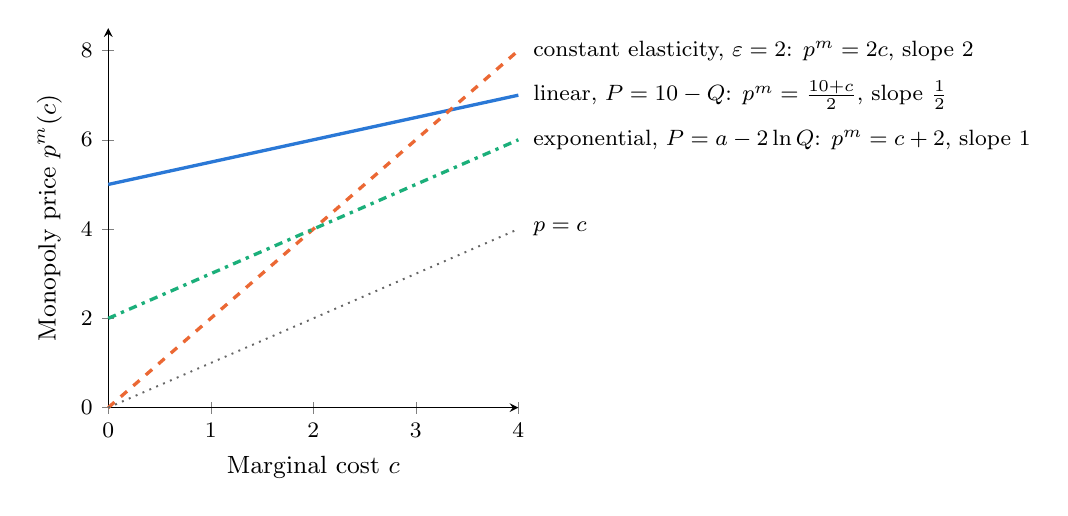
\begin{tikzpicture}
\definecolor{ptA}{HTML}{2A78D6}
\definecolor{ptB}{HTML}{EB6834}
\definecolor{ptC}{HTML}{1BAF7A}
\begin{axis}[
  width=0.56\textwidth, height=6.4cm,
  xmin=0, xmax=4, ymin=0, ymax=8.5,
  xlabel={Marginal cost $c$}, ylabel={Monopoly price $p^m(c)$},
  xtick={0,1,2,3,4}, ytick={0,2,4,6,8},
  tick label style={font=\footnotesize}, label style={font=\small},
  axis lines=left, clip=false, every axis plot/.append style={line width=1.2pt}]
  \addplot[domain=0:4, samples=2, color=ptA] {(10 + x)/2};
  \addplot[domain=0:4, samples=2, color=ptB, dashed] {2*x};
  \addplot[domain=0:4, samples=2, color=ptC, dash dot] {x + 2};
  \addplot[domain=0:4, samples=2, color=black!60, line width=0.7pt, dotted] {x};
  \node[anchor=west, font=\footnotesize, align=left] at (axis cs:4.05,8.0)
    {constant elasticity, $\varepsilon = 2$: $p^m = 2c$, slope $2$};
  \node[anchor=west, font=\footnotesize, align=left] at (axis cs:4.05,7.0)
    {linear, $P = 10 - Q$: $p^m = \frac{10 + c}{2}$, slope $\frac{1}{2}$};
  \node[anchor=west, font=\footnotesize, align=left] at (axis cs:4.05,6.0)
    {exponential, $P = a - 2\ln Q$: $p^m = c + 2$, slope $1$};
  \node[anchor=west, font=\footnotesize, align=left] at (axis cs:4.05,4.0)
    {$p = c$};
\end{axis}
\end{tikzpicture}
\caption{Monopoly price as a function of constant marginal cost for three demand curves. Linear demand
($a = 10$, $b = 1$) passes through one half of a cost change, exponential demand ($b = 2$) passes through all
of it, and constant-elasticity demand ($\varepsilon = 2$) passes through twice the change. The dotted line is
price equal to cost.}
\label{fig:02-pt-examples}
\end{figure}

\subsection{Conduct, curvature and rising marginal cost}\label{sec:02-pt-general}

We now allow imperfect competition of any degree and marginal cost that rises with output. The industry
satisfies the supply relation \eqref{eq:02-supply-relation} with conduct $\theta$, and a specific tax $t$ adds to
marginal cost. Write the supply relation with the \emph{marginal consumer surplus}
\begin{equation}\label{eq:02-ms}
ms(Q) = -QP'(Q) \ge 0 .
\end{equation}
The name comes from consumer surplus $CS(Q) = \int_0^Q P(x)\,\dd x - QP(Q)$, whose derivative is
$P - P - QP' = ms(Q)$. It is the gain in consumer surplus from one more unit of output. The supply relation then
reads $P(Q) - \theta\, ms(Q) = MC(Q) + t$: the markup equals conduct times the marginal consumer surplus. A
monopolist ($\theta = 1$) keeps its markup equal to the surplus it would hand to inframarginal consumers by
expanding.

\begin{assumption}[Pass-through under conduct]\label{ass:02-pt-general}
Inverse demand $P(Q)$ is twice continuously differentiable with $P' < 0$. Industry marginal cost $MC(Q)$ is
continuously differentiable with $MC' \ge 0$. Conduct $\theta \in [0, 1]$ does not vary with $t$. Equilibrium
output $Q(t)$ is positive, is continuous in $t$, and satisfies
\begin{equation}\label{eq:02-pt-supply}
P(Q) + \theta QP'(Q) = MC(Q) + t ,
\end{equation}
together with the stability condition
$\Lambda(Q) \equiv P'(Q) - \theta\, ms'(Q) - MC'(Q) < 0$.
\end{assumption}

As in \cref{ass:02-pt-monopoly}, the stability condition is the nonsingularity condition of the implicit function
theorem, and continuity keeps $Q(t)$ on one local branch of solutions. Hence $Q(t)$ is continuously differentiable.
The stability condition says that perceived marginal revenue $P - \theta\, ms$ cuts effective marginal cost from
above. It holds under monopoly by the second-order condition, and under symmetric Cournot competition by
\cref{ass:02-cournot} (see the proof of \cref{prop:02-pt-cournot}). Three elasticities summarize the primitives at the equilibrium. The demand elasticity is
$\varepsilon = -\frac{P}{QP'}$. The supply elasticity $\varepsilon_S = \frac{MC + t}{Q\, MC'}$ is the elasticity
of output with respect to effective marginal cost along the marginal-cost curve, and it is infinite when marginal
cost is flat. The term $\varepsilon_{ms} = \frac{ms}{Q\, ms'}$ is the elasticity of the inverse marginal-surplus
function, the reciprocal of the elasticity of $ms$ with respect to output \citep[p.~539]{WeylFabinger2013}.
Differentiating \eqref{eq:02-ms},
\begin{equation*}
ms'(Q) = -P'(Q) - QP''(Q) = -P'(Q)\Bigl(1 + \frac{QP''}{P'}\Bigr) = -P'(Q)\,(1 - \chi) ,
\end{equation*}
so $\frac{1}{\varepsilon_{ms}} = \frac{Q\,ms'}{ms} = \frac{-QP'(1 - \chi)}{-QP'} = 1 - \chi$. Exponential demand has
$\chi = 1$, a constant marginal consumer surplus, and $\frac{1}{\varepsilon_{ms}} = 0$.

\begin{proposition}[Pass-through under conduct, \citealp{WeylFabinger2013}]\label{prop:02-pt-general}
Under \cref{ass:02-pt-general},
\begin{equation}\label{eq:02-pt-general}
\rho = \frac{\dd P}{\dd t} = \frac{1}{1 + \frac{\varepsilon - \theta}{\varepsilon_S} + \frac{\theta}{\varepsilon_{ms}}}
= \frac{1}{1 + \theta(1 - \chi) + \frac{\varepsilon - \theta}{\varepsilon_S}} ,
\end{equation}
and the denominator is positive.
\end{proposition}

\begin{proof}
\emph{Step 1.} Differentiate $P(Q) - \theta\, ms(Q) = MC(Q) + t$ with respect to $t$:
\begin{equation*}
\bigl[P'(Q) - \theta\, ms'(Q)\bigr]\frac{\dd Q}{\dd t} = MC'(Q)\frac{\dd Q}{\dd t} + 1 .
\end{equation*}
Collecting terms gives $\Lambda\frac{\dd Q}{\dd t} = 1$, so $\frac{\dd Q}{\dd t} = \frac{1}{\Lambda} < 0$.

\emph{Step 2.} The price moves along the demand curve, so
\begin{equation*}
\rho = P'(Q)\frac{\dd Q}{\dd t} = \frac{P'}{P' - \theta\, ms' - MC'} = \frac{1}{1 - \theta\frac{ms'}{P'} - \frac{MC'}{P'}} .
\end{equation*}

\emph{Step 3.} The demand term is $-\frac{ms'}{P'} = 1 - \chi = \frac{1}{\varepsilon_{ms}}$ by the computation
above.

\emph{Step 4.} For the cost term, the definitions of the two elasticities give
$MC' = \frac{MC + t}{Q\varepsilon_S}$ and $\lvert P'\rvert = \frac{P}{\varepsilon Q}$. Hence
\begin{equation*}
-\frac{MC'}{P'} = \frac{MC'}{\lvert P'\rvert} = \frac{MC + t}{Q\varepsilon_S}\cdot\frac{\varepsilon Q}{P}
= \frac{\varepsilon}{\varepsilon_S}\cdot\frac{MC + t}{P} .
\end{equation*}

\emph{Step 5.} The Lerner form of \eqref{eq:02-pt-supply} is $\frac{P - MC - t}{P} = \frac{\theta}{\varepsilon}$,
as in \eqref{eq:02-theta-lerner}, so $\frac{MC + t}{P} = \frac{\varepsilon - \theta}{\varepsilon}$. Substituting into
Step 4 gives $-\frac{MC'}{P'} = \frac{\varepsilon - \theta}{\varepsilon_S}$.

\emph{Step 6.} Steps 2 to 5 give \eqref{eq:02-pt-general}. The denominator equals $\frac{\Lambda}{P'}$, a ratio
of two negative numbers, so it is positive.
\end{proof}

Step 2 has a geometric reading. With flat marginal cost, pass-through is the slope of inverse demand divided by
the slope of perceived marginal revenue, $\frac{P'}{P'(1 + \theta(1 - \chi))}$. A tax shifts the effective
marginal cost line up by $t$. Output falls until perceived marginal revenue has risen by $t$, and price rises by
the demand slope times the output change. When perceived marginal revenue is steep relative to demand, a small
output cut absorbs the tax and price rises little. Under exponential demand, marginal consumer surplus is constant, so
perceived marginal revenue is parallel to demand and price rises one for one. With rising marginal cost,
effective marginal cost also falls as output contracts. A smaller output cut then restores the supply relation,
and price rises less under every conduct.

\citet[eq.~(2), p.~548]{WeylFabinger2013} derive \eqref{eq:02-pt-general} for symmetric imperfect competition
and extend it to conduct that varies with output. Their denominator adds the term $\frac{\theta}{\varepsilon_\theta}
= Q\,\theta'(Q)$, where $\varepsilon_\theta = \frac{\theta}{Q\,\theta'(Q)}$ is the inverse of the elasticity of
conduct with respect to output. The version here assumes constant $\theta$, so this term vanishes.

\begin{corollary}[Special cases]\label{cor:02-pt-cases}
Under \cref{ass:02-pt-general}:
\begin{enumerate}[label=(\roman*)]
\item Price taking ($\theta = 0$) gives $\rho = \frac{\varepsilon_S}{\varepsilon_S + \varepsilon} \le 1$, with
  equality if and only if marginal cost is flat.
\item Flat marginal cost ($\varepsilon_S = \infty$) gives
  \begin{equation}\label{eq:02-pt-flat}
  \rho = \frac{1}{1 + \theta(1 - \chi)} .
  \end{equation}
\item Monopoly with flat marginal cost gives $\rho = \frac{1}{2 - \chi}$, which is \cref{prop:02-pt-monopoly}.
\item Symmetric Cournot competition among $N$ firms with flat marginal cost gives
  $\rho = \frac{N}{N + 1 - \chi}$. Linear demand gives $\frac{N}{N + 1}$, and constant elasticity gives
  $\frac{N\varepsilon}{N\varepsilon - 1} > 1$.
\item Monopoly with linear demand $P = a - bQ$ and linear marginal cost $MC = c_0 + kQ$ gives
  $\rho = \frac{b}{2b + k}$.
\end{enumerate}
\end{corollary}

\begin{proof}
(i) Setting $\theta = 0$ in \eqref{eq:02-pt-general} gives
$\rho = \frac{1}{1 + \frac{\varepsilon}{\varepsilon_S}} = \frac{\varepsilon_S}{\varepsilon_S + \varepsilon}$. The
same answer follows directly. A competitive industry with demand $Q(p)$ sets $p = MC(Q(p)) + t$.
Differentiating, $\rho = MC'(Q)\,Q'(p)\,\rho + 1$, so
\begin{equation*}
\rho = \frac{1}{1 + MC'\,\lvert Q'\rvert} = \frac{1}{1 + \frac{p}{Q\varepsilon_S}\cdot\frac{\varepsilon Q}{p}}
= \frac{\varepsilon_S}{\varepsilon_S + \varepsilon} ,
\end{equation*}
where the middle step uses $p = MC + t$. The ratio is below one whenever $\varepsilon_S < \infty$.

(ii) The term $\frac{\varepsilon - \theta}{\varepsilon_S}$ vanishes when $\varepsilon_S = \infty$.

(iii) Set $\theta = 1$ in \eqref{eq:02-pt-flat}. By \cref{lem:02-chi-direct} this equals
\eqref{eq:02-pt-logcurv}.

(iv) Each firm's first-order condition is $P + q_iP'(Q) = c + t$. Summing over the $N$ firms and dividing by
$N$ gives $P + \frac{1}{N}QP'(Q) = c + t$, the supply relation with $\theta = \frac{1}{N}$. Then
\eqref{eq:02-pt-flat} gives
\begin{equation*}
\rho = \frac{1}{1 + \frac{1 - \chi}{N}} = \frac{N}{N + 1 - \chi} .
\end{equation*}
Linear demand has $\chi = 0$. Constant elasticity has $\chi = 1 + \frac{1}{\varepsilon}$, so
$N + 1 - \chi = N - \frac{1}{\varepsilon}$ and $\rho = \frac{N\varepsilon}{N\varepsilon - 1}$. An interior
equilibrium requires $N\varepsilon > 1$.

(v) Here $\chi = 0$, and $\frac{\varepsilon - 1}{\varepsilon_S} = \frac{MC'}{\lvert P'\rvert} = \frac{k}{b}$ by
Steps 4 and 5 of the proof of \cref{prop:02-pt-general}. So $\rho = \frac{1}{2 + \frac{k}{b}} = \frac{b}{2b + k}$.
Directly, $a - 2bQ = c_0 + kQ + t$ gives $Q = \frac{a - c_0 - t}{2b + k}$ and $\frac{\dd P}{\dd t} = -b\frac{\dd Q}{\dd t} = \frac{b}{2b + k}$.
\end{proof}

Part (i) is the textbook incidence result for competitive markets. The side of the market with the smaller
elasticity bears more of the tax. Part (iv) shows that Cournot pass-through approaches one as $N$ grows, for any
fixed curvature. With constant elasticity it approaches one from above, so a more competitive industry passes
through less. \Cref{fig:02-pt-curvature} plots \eqref{eq:02-pt-flat} against curvature for four values of
conduct.

\begin{figure}[htbp]
\centering
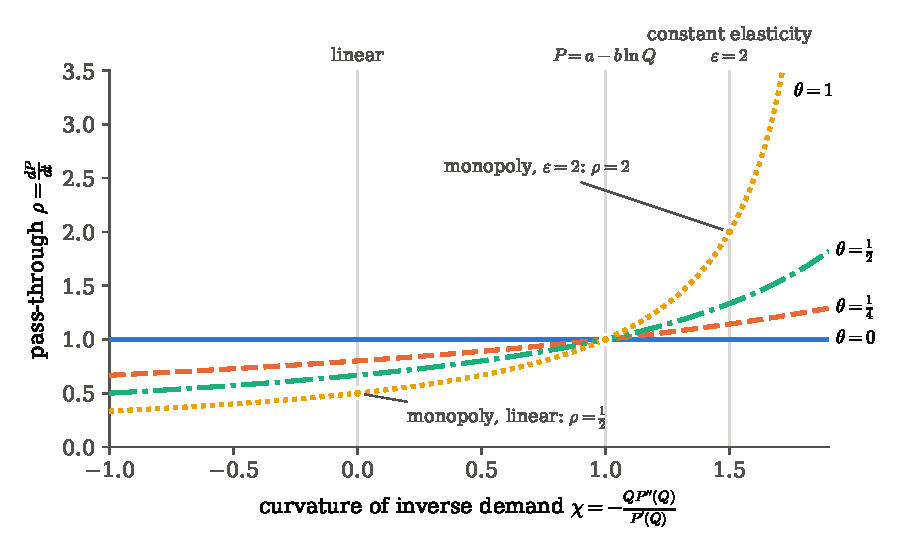
\includegraphics[width=0.86\textwidth]{figures/ch02/passthrough_curvature.pdf}
\caption{Pass-through with flat marginal cost, $\rho = \frac{1}{1 + \theta(1 - \chi)}$, against the curvature
of inverse demand for four values of conduct. All curves cross at $\chi = 1$ (exponential demand), where
$\rho = 1$ under every conduct. To the left of $\chi = 1$ market power lowers pass-through. To the right it
raises pass-through. The dots mark monopoly with linear demand ($\rho = \frac{1}{2}$), exponential demand
($\rho = 1$) and constant elasticity $\varepsilon = 2$ ($\rho = 2$). The monopoly curve is cut at
$\rho = 3.5$.}
\label{fig:02-pt-curvature}
\end{figure}

The figure shows the identification problem at a glance. Under competition with flat marginal cost, pass-through
is one for every demand curve. Market power rotates the line around the point $\chi = 1$. A pass-through above
one can come from strong market power with mild convexity or from weak market power with strong convexity.

\begin{corollary}[What pass-through reveals]\label{cor:02-pt-reveal}
Under \cref{ass:02-pt-general}:
\begin{enumerate}[label=(\roman*)]
\item Under price taking, $\rho \le 1$ for every demand curve and every nondecreasing marginal cost. A
  pass-through above one therefore rejects price taking.
\item With flat marginal cost, $\rho$ identifies only the product
  \begin{equation}\label{eq:02-pt-kappa}
  \theta(\chi - 1) = 1 - \frac{1}{\rho} .
  \end{equation}
  Every $\theta \in (0, 1]$ is consistent with every observed $\rho > 0$ for a suitable curvature. Price taking
  ($\theta = 0$) is consistent only with $\rho = 1$, whatever the curvature.
\item With rising marginal cost, $\theta(\chi - 1) = 1 - \frac{1}{\rho} + \frac{\varepsilon - \theta}{\varepsilon_S}
  \ge 1 - \frac{1}{\rho}$. Rising marginal cost lowers pass-through for given conduct and curvature, so it
  strengthens the rejection in (i). Price taking is then consistent with every $\rho \in (0, 1)$ for a suitable
  supply elasticity.
\item With constant-elasticity demand and flat marginal cost, $\theta = \varepsilon\bigl(1 - \frac{1}{\rho}\bigr)$.
  An estimate of the demand elasticity then converts pass-through into conduct.
\end{enumerate}
\end{corollary}

\begin{proof}
(i) is \cref{cor:02-pt-cases}(i). (ii) Rearrange \eqref{eq:02-pt-flat} as $\frac{1}{\rho} = 1 - \theta(\chi - 1)$.
The data enter only through $\rho$, so only the product $\theta(\chi - 1)$ is identified. Given $\rho$ and
$\theta > 0$, the curvature $\chi = 1 + \frac{1}{\theta}\bigl(1 - \frac{1}{\rho}\bigr)$ reproduces $\rho$. This
curvature satisfies the stability condition $1 + \theta(1 - \chi) = \frac{1}{\rho} > 0$, and under monopoly it
satisfies $\chi < 2$. A value $\rho \le 1$ requires $\chi \le 1$ when $\theta > 0$. With $\theta = 0$ the left
side of \eqref{eq:02-pt-kappa} is zero for every $\chi$, so $\rho = 1$. (iii) Rearrange \eqref{eq:02-pt-general}.
The added term is nonnegative because $\varepsilon \ge \theta$ whenever $P \ge MC + t$. With $\theta = 0$,
\cref{cor:02-pt-cases}(i) gives $\rho = \frac{\varepsilon_S}{\varepsilon_S + \varepsilon}$, which takes every
value in $(0, 1)$ as $\varepsilon_S$ ranges over $(0, \infty)$. (iv) Constant elasticity has $\chi - 1 = \frac{1}{\varepsilon}$.
Substitute into \eqref{eq:02-pt-kappa}.
\end{proof}

Part (i) is the robust content of a pass-through test. It needs no assumption on demand, and it needs only that
marginal cost does not fall with output. Two caveats apply. The price must be a product price, since a price
index can move for reasons of composition (\cref{sec:02-pt-composition}). The shifter must also move cost alone,
since a tax that shifts demand (for example through cross-border shopping) breaks the derivation. Part (ii) says
that a single market-wide cost shock moves the equilibrium along one demand curve, and that this movement cannot
separate conduct from curvature. \Cref{fig:02-pt-identified} draws the set of pairs $(\chi, \theta)$ consistent
with an illustrative pass-through of $1.07$. Separating the two requires an assumption on curvature, as in part
(iv), or variation that changes the slope of demand at a given price. \Cref{ch:conduct} develops both routes and
applies them to Sumner's cigarette data and to sugar refining.

\begin{figure}[htbp]
\centering
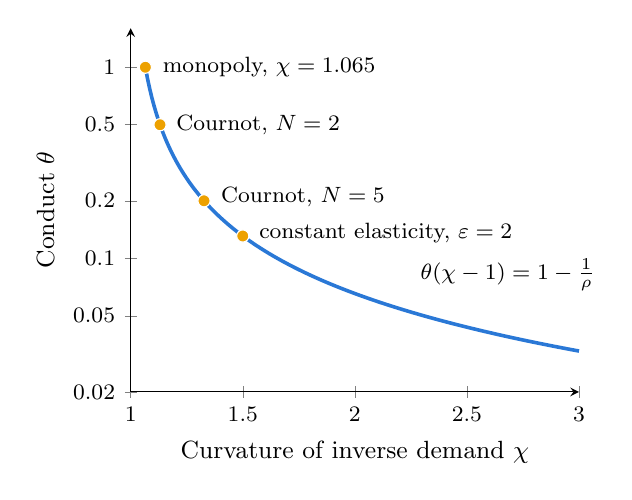
\begin{tikzpicture}
\definecolor{ptA}{HTML}{2A78D6}
\definecolor{ptD}{HTML}{EDA100}
\begin{axis}[
  width=0.6\textwidth, height=6.2cm,
  xmin=1, xmax=3, ymin=0.02, ymax=1.6, ymode=log,
  xlabel={Curvature of inverse demand $\chi$}, ylabel={Conduct $\theta$},
  xtick={1,1.5,2,2.5,3}, ytick={0.02,0.05,0.1,0.2,0.5,1},
  yticklabels={$0.02$,$0.05$,$0.1$,$0.2$,$0.5$,$1$},
  tick label style={font=\footnotesize}, label style={font=\small},
  axis lines=left, clip=false]
  \addplot[domain=1.0654:3, samples=200, color=ptA, line width=1.3pt] {0.0654206/(x - 1)};
  \addplot[only marks, mark=*, mark size=2.2pt, color=ptD, draw=white]
    coordinates {(1.0654,1) (1.1308,0.5) (1.3271,0.2) (1.5,0.13084)};
  \node[anchor=west, font=\footnotesize] at (axis cs:1.10,1.0) {monopoly, $\chi = 1.065$};
  \node[anchor=west, font=\footnotesize] at (axis cs:1.16,0.5) {Cournot, $N = 2$};
  \node[anchor=west, font=\footnotesize] at (axis cs:1.36,0.21) {Cournot, $N = 5$};
  \node[anchor=west, font=\footnotesize] at (axis cs:1.53,0.135) {constant elasticity, $\varepsilon = 2$};
  \node[anchor=south west, font=\footnotesize] at (axis cs:2.25,0.06) {$\theta(\chi - 1) = 1 - \frac{1}{\rho}$};
\end{axis}
\end{tikzpicture}
\caption{Pairs of demand curvature and conduct consistent with an illustrative pass-through $\rho = 1.07$ when
marginal cost is flat. Every point on the curve satisfies $\theta(\chi - 1) = 1 - \frac{1}{1.07} \approx 0.065$.
Symmetric Cournot with $N$ firms ($\theta = \frac{1}{N}$) fits with $\chi = 1 + 0.065N$. A constant-elasticity
demand with elasticity $\varepsilon$ has $\chi = 1 + \frac{1}{\varepsilon}$ and fits with
$\theta = 0.065\varepsilon$. The vertical axis is logarithmic.}
\label{fig:02-pt-identified}
\end{figure}

\subsection{Firm-specific versus industry-wide cost shocks in Cournot}\label{sec:02-pt-cournot}

So far a tax raised every firm's cost together. Many cost shocks hit one firm only: a local wage increase, a
plant outage, a merger's cost savings, or an exchange-rate shock to one importer. In a homogeneous-good market
all firms charge one price, and the question becomes how much that price responds to one firm's cost.

The linear Cournot model of \cref{ex:02-linear-cournot} gives the answer in closed form. With $P = a - bQ$ and
constant costs $c_1, \dots, c_N$,
\begin{equation*}
P^* = \frac{a + \sum_j c_j}{N + 1}, \qquad q_i^* = \frac{a - (N + 1)c_i + \sum_j c_j}{b(N + 1)} .
\end{equation*}
A rise in $c_i$ alone and a common rise $\dd c_j = \dd c$ for all $j$ give
\begin{equation*}
\frac{\dd P^*}{\dd c_i} = \frac{1}{N + 1}, \qquad \frac{\dd q_i^*}{\dd c_i} = -\frac{N}{b(N + 1)}, \qquad
\frac{\dd q_j^*}{\dd c_i} = \frac{1}{b(N + 1)} \;\; (j \ne i), \qquad \frac{\dd P^*}{\dd c} = \frac{N}{N + 1} .
\end{equation*}
Firm $i$'s margin $P^* - c_i$ falls by $\frac{N}{N + 1}$ per dollar of its own
cost increase, so the firm absorbs most of a firm-specific shock. The next result extends these formulas to
nonlinear demand.

\begin{proposition}[Cournot pass-through]\label{prop:02-pt-cournot}
Let (C1) and (C3) of \cref{ass:02-cournot} hold with constant marginal costs $c_1, \dots, c_N$, let all $N$ firms
be active, and suppose $P'(Q) + q_jP''(Q) < 0$ at the equilibrium for every $j$ (as (C2) guarantees).
Let $s_i = \frac{q_i}{Q}$ and let $\chi$ be the curvature \eqref{eq:02-chi} at the equilibrium output. Then
$N + 1 - \chi > 0$, and
\begin{equation}\label{eq:02-pt-cournot}
\frac{\dd P}{\dd c_i} = \frac{1}{N + 1 - \chi}, \qquad \frac{\dd P}{\dd c} = \frac{N}{N + 1 - \chi}, \qquad
\frac{\dd q_i}{\dd c_i} = \frac{N - (1 - s_i)\chi}{P'(Q)\,(N + 1 - \chi)} < 0 ,
\end{equation}
where $\frac{\dd P}{\dd c}$ is the response to a common shock.
\end{proposition}

\begin{proof}
We use the replacement functions of \cref{sec:02-cournot}. With constant costs, $\tilde q_i(Q)$ solves
$P(Q) + qP'(Q) = c_i$, so $\tilde q_i(Q) = \frac{c_i - P(Q)}{P'(Q)}$ near the equilibrium. Differentiating
$P(Q) + qP'(Q) = c_i$ in $c_i$ at fixed $Q$ gives $\frac{\partial\tilde q_i}{\partial c_i} = \frac{1}{P'}$.
Differentiating it in $Q$ gives $P' + \tilde q_i'P' + \tilde q_iP'' = 0$, so
\begin{equation*}
\tilde q_j'(Q) = -\Bigl(1 + \frac{q_jP''}{P'}\Bigr) = -\Bigl(1 + \frac{q_j}{Q}\cdot\frac{QP''}{P'}\Bigr)
= -(1 - s_j\chi) .
\end{equation*}
By assumption $P' + q_jP'' < 0$ at the equilibrium. Dividing by $P' < 0$ gives $1 - s_j\chi > 0$ for every $j$.
Summing over $j$ and using $\sum_j s_j = 1$,
\begin{equation*}
1 - \sum_j \tilde q_j'(Q) = 1 + \sum_j (1 - s_j\chi) = N + 1 - \chi > 0 .
\end{equation*}
Industry output solves $\sum_j \tilde q_j(Q) = Q$. Since the derivative of $\sum_j \tilde q_j(Q) - Q$ in $Q$ is
nonzero, the implicit function theorem applies. Differentiating in $c_i$, as in the proof of
\cref{prop:02-cournot-cs}, gives
\begin{equation*}
\frac{\dd Q}{\dd c_i} = \frac{\frac{\partial\tilde q_i}{\partial c_i}}{1 - \sum_j \tilde q_j'(Q)} .
\end{equation*}
Hence $\frac{\dd Q}{\dd c_i} = \frac{1}{P'(N + 1 - \chi)}$ and $\frac{\dd P}{\dd c_i} = P'\frac{\dd Q}{\dd c_i} = \frac{1}{N + 1 - \chi}$.
A common shock is the sum of $N$ firm-specific shocks, so $\frac{\dd P}{\dd c} = \sum_i\frac{\dd P}{\dd c_i} = \frac{N}{N + 1 - \chi}$.
For firm $i$'s own output, $q_i = \tilde q_i(Q)$ in equilibrium, so
\begin{equation*}
\frac{\dd q_i}{\dd c_i} = \frac{\partial\tilde q_i}{\partial c_i} + \tilde q_i'(Q)\frac{\dd Q}{\dd c_i}
= \frac{1}{P'}\Bigl[1 - \frac{1 - s_i\chi}{N + 1 - \chi}\Bigr]
= \frac{N - (1 - s_i)\chi}{P'(N + 1 - \chi)} .
\end{equation*}
The numerator equals $1 + \sum_{j \ne i}(1 - s_j\chi) > 0$, and $P' < 0$, so $\frac{\dd q_i}{\dd c_i} < 0$.
\end{proof}

Three features of \eqref{eq:02-pt-cournot} stand out. First, the price response to a firm-specific shock does
not depend on the firm's share. A large firm and a small firm move the price by the same amount after equal
cost increases. The direct effect on a firm's replacement output, $\frac{1}{P'}$, does not depend on its size, and
rivals respond only to total output. Second, the
common-shock pass-through equals \cref{cor:02-pt-cases}(iv) even with asymmetric costs. Third, the ratio of the
two is $N$ for any demand curve. A firm-specific shock moves the market price by only a fraction
$\frac{1}{N + 1 - \chi}$ of the shock, and the firm bears the rest through a lower margin.

The distinction matters for empirical work. A market-wide shifter, such as an excise tax, moves the industry
along the market demand curve. Its pass-through speaks to industry conduct and market demand curvature, as in
\cref{sec:02-pt-general}. A firm-specific shifter, such as a firm's own input price, moves the equilibrium along
the firm's residual demand curve, which includes rivals' supply responses. \citet{BakerBresnahan1988} use such
shifters to estimate residual demand directly (\cref{ch:conduct}). The distinction also matters for mergers.
The cost savings of a merger are specific to the merged firm, so the relevant pass-through is the
firm-specific one. Using an industry-wide rate would overstate how much of the savings reaches consumers
(\cref{ch:mergers}).

\subsection{Incidence}\label{sec:02-pt-incidence}

Pass-through determines who bears a tax. Consumer surplus is $CS = \int_0^Q P(x)\,\dd x - P(Q)Q$. Producer surplus
is variable profit, $PS = P(Q)Q - C(Q) - tQ$, where $C$ is industry variable cost with $C' = MC$ (as with
symmetric firms). Tax revenue is $R = tQ$.

\begin{proposition}[Incidence under conduct, {\citealp[pp.~546--548]{WeylFabinger2013}}]\label{prop:02-incidence}
Under \cref{ass:02-pt-general}, a small change in the specific tax changes surplus by
\begin{equation*}
\frac{\dd CS}{\dd t} = -\rho Q, \qquad \frac{\dd PS}{\dd t} = -\bigl[1 - (1 - \theta)\rho\bigr]Q .
\end{equation*}
When the producer burden is nonzero, the \emph{incidence ratio}, consumer burden divided by producer burden, is
\begin{equation}\label{eq:02-incidence}
I = \frac{\frac{\dd CS}{\dd t}}{\frac{\dd PS}{\dd t}} = \frac{\rho}{1 - (1 - \theta)\rho} .
\end{equation}
Total surplus $W = CS + PS + R$ satisfies $\frac{\dd W}{\dd t} = -\theta\rho Q + t\frac{\dd Q}{\dd t}$.
\end{proposition}

\begin{proof}
\emph{Consumers.} By Leibniz's rule,
\begin{equation*}
\frac{\dd CS}{\dd t} = P(Q)\frac{\dd Q}{\dd t} - \Bigl[P'(Q)Q + P(Q)\Bigr]\frac{\dd Q}{\dd t} = -QP'(Q)\frac{\dd Q}{\dd t} = -Q\rho ,
\end{equation*}
since $\rho = P'\frac{\dd Q}{\dd t}$.

\emph{Producers.} Differentiating $PS$,
\begin{equation*}
\frac{\dd PS}{\dd t} = P'Q\frac{\dd Q}{\dd t} + P\frac{\dd Q}{\dd t} - MC\frac{\dd Q}{\dd t} - Q - t\frac{\dd Q}{\dd t}
= Q(\rho - 1) + (P - MC - t)\frac{\dd Q}{\dd t} .
\end{equation*}
The supply relation \eqref{eq:02-pt-supply} gives $P - MC - t = -\theta QP'$, and $\frac{\dd Q}{\dd t} = \frac{\rho}{P'}$.
Hence $(P - MC - t)\frac{\dd Q}{\dd t} = -\theta QP'\cdot\frac{\rho}{P'} = -\theta\rho Q$, and
\begin{equation*}
\frac{\dd PS}{\dd t} = Q(\rho - 1) - \theta\rho Q = -Q\bigl[1 - (1 - \theta)\rho\bigr] .
\end{equation*}
Dividing the two derivatives gives \eqref{eq:02-incidence}.

\emph{Total surplus.} Revenue changes by $\frac{\dd R}{\dd t} = Q + t\frac{\dd Q}{\dd t}$. Adding the three derivatives,
\begin{equation*}
\frac{\dd W}{\dd t} = -\rho Q - Q + (1 - \theta)\rho Q + Q + t\frac{\dd Q}{\dd t} = -\theta\rho Q + t\frac{\dd Q}{\dd t} .
\qedhere
\end{equation*}
\end{proof}

\citet[p.~546]{WeylFabinger2013} credit \citet{AtkinDonaldson2012} with first deriving the formula for
$\frac{\dd PS}{\dd t}$, which extends the monopoly case to general conduct.

The special cases are instructive. Under price taking, $I = \frac{\rho}{1 - \rho}$. With
$\rho = \frac{\varepsilon_S}{\varepsilon_S + \varepsilon}$ from \cref{cor:02-pt-cases}(i), this is
$I = \frac{\varepsilon_S}{\varepsilon}$, the classic rule that the burden falls on the less elastic side. With flat
marginal cost, competitive producers bear nothing. Under monopoly, $\frac{\dd PS}{\dd t} = -Q$ whatever the demand
curve, which is the envelope theorem at work (\cref{app:math}), and $I = \rho$. Consumers bear more than the
monopolist exactly when $\rho > 1$. With linear demand, flat cost and conduct $\theta$, $\rho = \frac{1}{1 + \theta}$
and
\begin{equation*}
I = \frac{\frac{1}{1 + \theta}}{1 - \frac{1 - \theta}{1 + \theta}} = \frac{\frac{1}{1 + \theta}}{\frac{2\theta}{1 + \theta}}
= \frac{1}{2\theta} .
\end{equation*}
A linear monopoly ($\theta = 1$) puts one third of the private burden on consumers, and a symmetric Cournot duopoly
($\theta = \frac{1}{2}$) splits it equally.

Market power changes incidence in two ways that competitive analysis misses. First, consumers can bear more than
the full tax ($\rho > 1$) while producers still lose. With constant elasticity $\varepsilon = 2$, a monopolist
passes through $\rho = 2$, consumers lose $2Q$ per unit of tax and the monopolist loses $Q$. Second, producers
can gain from a tax. The producer burden is negative when $\rho > \frac{1}{1 - \theta}$. With flat marginal cost
this condition reduces to $\theta(2 - \chi) < 0$, that is $\chi > 2$ for $\theta > 0$. Monopoly rules this out
through its second-order condition, but oligopoly with $\theta < 1$ allows $2 < \chi < 1 + \frac{1}{\theta}$.
In symmetric Cournot with constant elasticity,
\begin{equation*}
1 - \Bigl(1 - \frac{1}{N}\Bigr)\frac{N\varepsilon}{N\varepsilon - 1} = \frac{\varepsilon - 1}{N\varepsilon - 1} ,
\end{equation*}
which is negative when $\frac{1}{N} < \varepsilon < 1$. A common cost increase then raises industry profit. It
pushes output toward the level that maximizes joint profit, which the firms could not reach on their own.

The total-surplus formula adds a third difference. Under competition the first tax dollar has no deadweight cost,
because $\frac{\dd W}{\dd t} = 0$ at $t = 0$ when $\theta = 0$. Under market power the first dollar already costs
$\theta\rho Q$, because output starts below its efficient level (\cref{sec:02-welfare}). Linear monopoly loses
$\frac{Q}{2}$ of surplus per unit of tax at $t = 0$, half of the revenue raised. \citet[pp.~537 and
546]{WeylFabinger2013} state that this excess burden is $\rho$ per unit of revenue under monopoly and positive
whenever $\theta > 0$. We add the total-surplus formula itself, which also holds at $t > 0$.

\begin{remark}[Ad valorem taxes]\label{rem:02-pt-adval}
An \emph{ad valorem tax} at rate $t_a$ takes a fraction $t_a$ of the price. Firms receive $(1 - t_a)P$, and the
supply relation becomes $(1 - t_a)(P + \theta QP') = MC(Q)$, that is $P + \theta QP' = \frac{MC(Q)}{1 - t_a}$.
An ad valorem tax therefore scales effective marginal cost by $\frac{1}{1 - t_a}$. At $t_a = 0$ a small rate
$\dd t_a$ raises effective marginal cost by $MC\,\dd t_a$, so $\frac{\dd P}{\dd t_a} = \rho\, MC$. A specific tax
$\dd t = P\,\dd t_a$ raises the same revenue to first order and raises price by $\rho P\,\dd t_a$. At $t_a = 0$
the Lerner form gives $MC = (1 - \frac{\theta}{\varepsilon})P$, so the ad valorem tax raises price less per dollar
of revenue whenever $\theta > 0$. Under competition the two taxes coincide to first order. The incidence formulas for ad valorem taxes
are left to \cref{sec:02-exercises}.
\end{remark}

\subsection{Measured prices and composition}\label{sec:02-pt-composition}

Pass-through regressions often use a price index, an average across products, as the dependent variable. The
index can move even when no product's price moves, because the mix of products bought changes.

\begin{remark}[Composition bias]\label{rem:02-pt-composition}
Let the observed price be the quantity-weighted average $\bar p = \sum_j w_jp_j$, with weights $w_j \ge 0$
summing to one. Differentiating with respect to the tax,
\begin{equation}\label{eq:02-pt-composition}
\frac{\dd \bar p}{\dd t} = \underbrace{\sum_j w_j\frac{\dd p_j}{\dd t}}_{\text{price effect}}
+ \underbrace{\sum_j p_j\frac{\dd w_j}{\dd t}}_{\text{composition effect}} .
\end{equation}
The first term is the average of product-level pass-through. The second term is nonzero whenever the tax changes
the mix of purchases. A regression of $\bar p$ on $t$ estimates the sum.
\end{remark}

A specific tax tends to make the composition effect positive. It raises every price by a similar dollar amount,
which is a larger percentage of a cheap product's price. Suppose a cheap and an expensive product have prices
$p_L < p_H$, and each price rises one for one with the tax. The relative price $\frac{p_H + t}{p_L + t}$ has
derivative $\frac{p_L - p_H}{(p_L + t)^2} < 0$ in $t$, so the expensive product becomes relatively cheaper. If
buyers respond to relative prices, the weight $w_H$ rises, and the composition effect
$(p_H - p_L)\frac{\dd w_H}{\dd t}$ is positive. A numerical illustration makes the size concrete. Let $p_L = 1$,
$p_H = 2$ and $w_H = 0.5$, and let a tax of $0.10$ raise both prices by $0.10$ and $w_H$ to $0.52$. The index
rises from $1.50$ to $0.48 \times 1.10 + 0.52 \times 2.10 = 1.62$, so the measured pass-through is $1.2$ although
each product's pass-through is exactly one.

The bias pushes a test toward rejecting price taking, because it can create $\hat\rho > 1$ from product-level
pass-through equal to one. The remedies are to estimate pass-through at the product level, or to use a
fixed-weight index $\sum_j w_j^0 p_j$ that holds the weights at their pre-tax values. The same logic runs in the
opposite direction when demand peaks. \citet{NevoHatzitaskos2005} study canned tuna, whose average price falls
during Lent although demand is high. They argue that a shift of purchases toward cheaper products explains much
of the fall in the average price paid. In their supermarket data, the Lent coefficient is $-1.78$ cents per ounce
for the quantity-weighted tuna price index and $-0.51$ for a fixed-weight index \citep[p.~13 and
Table~3]{NevoHatzitaskos2005}.
\Cref{ch:conduct} returns to composition as one of the three standard critiques of Sumner's cigarette-tax test.

Pass-through thus carries information about market power, but only jointly with the curvature of demand and the
slope of marginal cost. Pass-through above one is hard to reconcile with price taking. Beyond that, a pass-through
estimate must be combined with an assumption or a second source of variation before it reveals conduct. The
incidence of taxes, the consumer benefits of cost savings and the price effects of mergers all inherit this
dependence on curvature.
